\section{Turing Pattern Formation}
Nature offers a wide varge of examples of bialogical potterns, from animal pigmentation to shells, shim, wings and skeletal stunctures. Patterns are composed of spatially heteragenesons structures which may emerge owing to several (bialgical) reasons. These could arise in systems in which chemicals react with each other and also underswent diffusion - a mechonism which is termed diffusiondriven instability. This is the besis of the so called Turing patterns.
\begin{center}
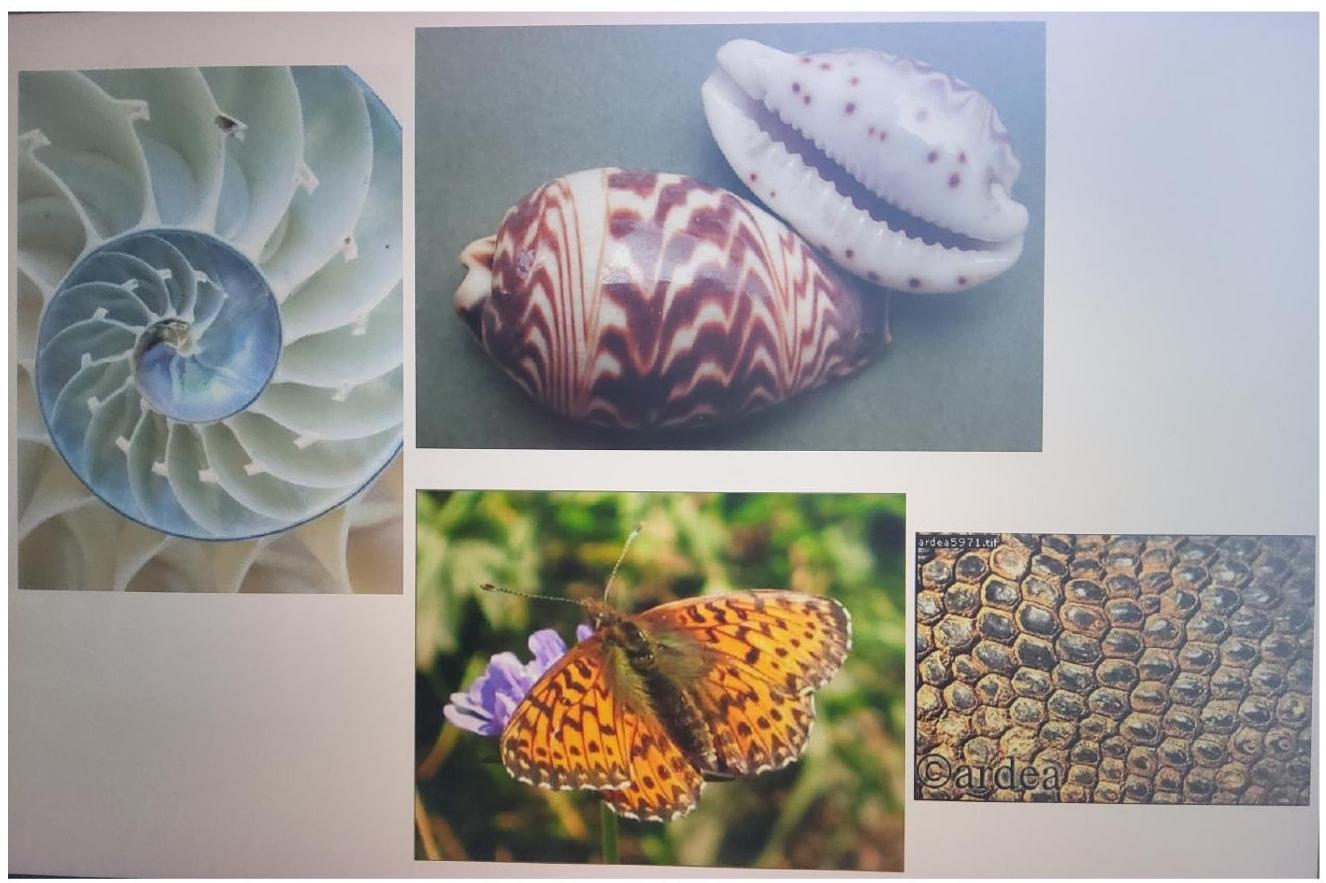
\includegraphics[width=\textwidth]{2025_10_17_3cf351a4349ae3691080g-01}
\end{center}

Turing potterns and istobility are related to symmetry breaking in non-equilibrium systems and represent an example of emergent pattern, namely, a structure that energes from the combination of processes, which per se do not possess any property related to the pottern itself.

In 1952 Alow Turing (logicion, computer scientist, code breaker and mothematicion) propased a methematical model which was able to show emengent patterns (A.M. Turing, the chemical basis of morphogenesis, Philos. Trous. R. Soc. London B $237,37-72,(1952)$ ).

Turing showed that when some chemicals react with each other and diffuse appropriatcly, then spotially heterogencous potterns con emerge (diffurion-driven instability), if some conditions are met.

One chemical species
Let us consider the case with one chemical species, diffusing in a one-dimensional space. We could consider the reactions

$$
\left.\begin{array}{l}
3 U \underset{k_{-}}{\stackrel{k_{+}}{\rightleftarrows}} 2 U \\ 
\phi \underset{\mu_{-}}{\mu_{+}} U
\end{array}\right\} \rightarrow \dot{u}=-k_{+} u^{3}+u_{-} u^{2}-\mu_{-} u+\mu_{+}
$$

which invalve only the pecies $U(u$ is is concentration).
For the sate of generality, let's assume that the chemical $U$ is being produced at wate $f(u)$ (typically a polynomial or a sationd function of $u$ ). If we include diffusion
(1) \quad \frac{\partial u}{\partial t}=D \frac{\partial^{2} u}{\partial x^{2}}+f(u)

Where $D>0$ is the diffusion coefficient. Eq. (1) is a reaction-diffusion equation.
We also assume that $U$ diffuses in a domain $(0,1)$ and that
(2) $u(0, t)=u_{0}=u(L, t)$ for any $t$

These are called Dirichlet boundary conditions. If there is a spetially uniform stationary state $u$. for $u$, then we also have $\lim _{t} u(x, t)=u_{0}$ and $f\left(u_{0}
ight)=0$.
Is this state stable? In general this is a hard question, but we can check whether $u_{0}$ is linearly stable. To check This we have to determine the effect of a small perturbation.
$\hat{u}(x, t)=u(x, t)-u_{0} \quad\left(|
\hat{u}| \ll u_{0}
ight)$. Exponding $f$ in a Taylor series we get (only linear terms) from ep. (1)
(3) \quad \frac{\partial \hat{u}}{\partial t}=\Delta \frac{\partial^{2} \hat{u}}{\partial x^{2}}+f^{\prime}
\left(u_{0}
ight) \hat{u} \quad \hat{u}(0, t)=0=\hat{u}(L, t)$
where we assumed $f
\left(u_{0}
ight)=0$ and $f^{\prime}
\left(u_{0}
ight) \neq 0$. Without space $(D=0)$ we get
(4) $\hat{u}(x, t)=\hat{u}_{0} e^{f^{\prime}
\left(u_{0}
ight) t}$
$\hat{u}_{0}$ is the initial perturbation. Of course, the steady state is stable if $f^{\prime}
\left(u_{0}
ight)<0$. If $D>0$, then ep. (3) can be solved via separation of variables: $\hat{u}(x, t)=h(x) k(t)$. Thus we get from ep. (3)

$$ 
\begin{aligned}
\left(\partial_{t} k\right) h & =D k\left(\partial_{x}^{2} h\right)+f^{\prime}
\left(u_{0}
ight) k h \ 
\frac{\partial t k}{k} & =D \frac{\partial_{x}^{2} h}{h}+f^{\prime}
\left(u_{0}
ight)
\end{aligned}
$$

because the l.h.s. depends on $t$ only and the 2.h.s. on $x$ only, it must be

$$ 
\underbrace{\frac{\partial_{t} k}{k}}_{a}=\overbrace{\lambda=D \frac{\partial_{x}^{2} h}{h}+f^{\prime}
\left(u_{0}
ight)}^{b}
$$

Where $\lambda$ is constant independent of time and pace
a) $\partial_{t} k=\lambda k \Rightarrow k(t)=k_{0} e^{\lambda t}$
b) $\partial_{x x}^{2} h=\underbrace{\frac{\lambda-f^{\prime}
\left(u_{0}
ight)}{D}}_{-\rho^{2}} h \Rightarrow h(x)=A \sin (\rho x)+B \cos (\rho x)$

From the B.C. in ep. (2) we obtain $h(0)=0 \Rightarrow B=0$ and also $h(L)=0 \Rightarrow \rho=\frac{n \pi}{L}$ for any $n=1,2 \ldots$
Hence the modes


\begin{equation*} 
\lambda_{u}=f^{\prime}
\left(u_{0}
ight)-D\left(\frac{n \pi}{L}
ight)^{2} \tag{5}
\end{equation*} 

$$ 
n=1,2, \cdots
$$

Because the ep. is linear, we can sum all the mades and get the final solution as a Fourier series:
(6) $\hat{u}(x, t)=\sum_{n=1}^{\infty} a_{n} \sin \left(\frac{n \pi_{x}}{L}\right) e^{\lambda_{m} t} \quad \hat{u}(0, t)=0=\hat{u}(L, t)$
where $a_{n}$ are determined to sotisfy the imitial condition for the pert. Note from (5) that, even if $f^{\prime}
\left(u_{0}
ight)>0$ ( $u_{0}$ is unstable), then $\Delta>f^{\prime}
\left(u_{0}
ight)\left(\frac{L}{\pi}
ight)^{2}$ (for fixed domain size L) implies $\lambda_{n}<0$. Therefore, all terms in ep. (6) with $a_{n} \neq 0$ have an expon. decay, hence $\hat{u} \rightarrow 0$ as $t \rightarrow \infty$.
In this cose the state $u_{0}$ is stabilized by diffusion, even when it is unstable, if $D$ is sufficiently large. D counst destabilize the solution.

\section*{Exercize:}
If B.C. are zero-flux at the boundaries $\left(\frac{\partial u}{\partial x}(0)=0=\frac{\partial u}{\partial x}(L)\right.$, Neumann B.C.) the zeroth made could still grow, but all the others decay exponentially so there camot be any spotial heterogeneity for longe $D$. Same arguments still hald for periodic B.C.

Obs: Notice that diffusivity is not always able to stabilize.
If we fix $D$ and increase $L$ when $f^{\prime}
\left(u_{0}
ight)>0$, then for rufficiently lorge domain sizes $\left(L>\sqrt{\frac{\Delta \pi^{2}}{f^{\prime}
\left(n_{0}
ight)}}
\right)$ we still get $\lambda_{n}>0$. The effect of diffusion depends on the domain.

Two on more chemical species

From the previous rection we have learnt that diffusion is able to smooth out inhomagencities, thus stabilizing processes. This ogrees with other phenomena, e.g., diffusion of heat within a finite domain.
Tursing understood that if there are more than one interacting species, this is not necessarily the cose and diffusion may destabilize homogeneous solutions.
Let $u(x, t)$ and $v(x, t)$ be the concentrations of two chemical species which satisfy the following reaction-diffusion equations in 1-d space:
(7) $\left\{
\begin{array}{l}\dot{u}=f(u, v)+D_{1} \frac{\partial^{2} u}{\partial x^{2}} \\ 
\dot{v}=g(u, v)+D_{2} \frac{\partial^{2} v}{\partial x^{2}}\end{array}\right. \quad$ with I.C. and B.C.
where $f$ and $g$ are smooth functions which describe the reactions between the two chemicals whose concentrations are given by $u$ and $v . D_{1}$ and $D_{2}$ are two diffusion constants. We assume that $x \in(0,1)$ (finite domain) and at the boundaries we impose zero-flux conditions (Neumann b.c.).

Let us assume that ep. (7) odmits a spatially uniform steady state, hence there exist $u_{0}$ and $v_{0}$ such that $f
\left(u_{0}, v_{0}
ight)=0=g
\left(u_{0}, v_{0}
ight)$. We now wish to derive conditions of linear stability for the state $\left(u_{0}, v_{0}
ight)$. For this we introduce small (spetiallydependent) perturbations $\hat{u}(x, t)=u(x, t)-u_{0}$ and $\hat{v}(x, t)=v(x, t)-v_{0}$ into of. (7) and expond $f$ and $g$ in Taylon series. We assive at (ucall that $f
\left(u_{0}, v_{0}
ight)=0, g
\left(u_{0}, v_{0}
ight)=0$ )
(8) $\quad\left\{
\begin{array}{l}\dot{\hat{u}}=\left.\frac{\partial f}{\partial u}\right|_{0} \hat{u}+\left.\frac{\partial f}{\partial v}\right|_{0} \hat{v}+D_{1} \frac{\partial^{2} \hat{u}}{\partial x^{2}} \\ 
\dot{\hat{v}}=\left.\frac{\partial g}{\partial u}\right|_{0} \hat{u}+\left.\frac{\partial g}{\partial v}\right|_{0} \hat{v}+D_{2} \frac{\partial^{2} \hat{v}}{\partial x^{2}}\end{array}\right.$
where $\left.\left.\frac{\partial f}{\partial u}\right|_{0} \equiv \frac{\partial f(u, v)}{\partial u}\right|_{\substack{u=u_{0} \v=v_{0}}}$ and the some for the rest. We con recost ep. (8) in the matrix form

$$ 
\binom{\partial_{t} \hat{u}}{\partial_{t} \hat{v}}=\underbrace{\left(\begin{array}{cc}
\left.\frac{\partial f}{\partial u}\right|_{0} & \left.\frac{\partial f}{\partial v}\right|_{0} \\ 
\left.\frac{\partial g}{\partial u}\right|_{0} & \frac{\partial g}{\left.\partial v\right|_{0}}\end{array}\right)}_{\equiv J_{0}}\binom{\hat{u}}{\hat{v}}+\underbrace{\left(\begin{array}{cc}
D_{1} & 0 \ 
0 & D_{2}\end{array}\right)\binom{\partial_{x}^{2} \hat{u}}{\partial_{x}^{2} \hat{v}}}_{\equiv D}
$$

or
(9) $\frac{\partial}{\partial t} \overrightarrow{\hat{u}}=J_{0} \overrightarrow{\hat{u}}+\Delta \partial_{x}^{2} \overrightarrow{\hat{u}}$

We carry out the anolysis of the previous section and look for a solution of the form


\begin{equation*} 
\vec{u}(x, t)=\vec{a} e^{\left(i k x+\lambda
\left(k^{2}
ight) t
ight)} \tag{10}
\end{equation*} 

where $\vec{a}$ is a constont vector. Subbing (10) into (9) we get

$$ 
\lambda \vec{a} e^{i k x+\lambda t}=J_{0} \vec{a} e^{i k x+\lambda t}-k^{2} D \vec{a} e^{i k x+\lambda t}
$$ 

which leads to the matrix equation
(11) $\left(J_{0}-k^{2} \Delta-\lambda 11\right) \vec{a}=\overrightarrow{0}$
where 11 is the unit $2 \times 2$ matrix and $\overrightarrow{0}=(0,0)^{T}$.

For non-trivial solutions to exist, we thus require that
(12) $\operatorname{det}
\left(J_{0}-k^{2} D-\lambda 1\right)=0$
this condition provides us equations for obtaining the eigenvalues $\lambda$ ( $0^{2}$ temporal growth rates) which are functions of $k^{2}$.
If we find $\operatorname{Re} \lambda>0$ for at least one eigenvalue then the solution is unstable.

In the previous section we showed that an ustable fixed point can be stobilized. Here we show that a stable homogencaus fixed point can be destabilized by diffusion: this is the core of Twring pattern formation (and the Turing's brilliont idea).
(1) A spatially-uniform steady state is linearly stable

Let us consider the cose with no diffusion $D_{1}=D_{2}=0$.
Then $\lambda$ is the eigenvolue of the matrix $J_{0}$ :

$$ 
\operatorname{det}
\left(J_{0}-\lambda 11\right)=\operatorname{det}\left(\begin{array}{cc}
\partial_{u} f-\lambda & \partial_{v} f \\ 
\partial_{u} g & \partial_{v} g-\lambda
\end{array}\right)=\left(\partial_{u} f-\lambda\right)\left(\partial_{v} g-\lambda\right)-\partial_{u} g \partial_{v} f=0
$$ 

or
(13) $\quad \lambda^{2}-\underbrace{\left(\partial_{u} f+\partial_{v} g
ight)}_{\text {sum of sols }} t+\underbrace{\partial_{u} f \partial_{v} g-\partial_{v} f \partial_{u} g}_{\text {prod. of sols. }}=0$

$$ 
\left[\lambda^{2}-\left(\lambda_{1}+\lambda_{2}
ight) \lambda+\lambda_{1} \lambda_{2}=0\right]
$$ 

For the partially uniform steady state to be stable, both eigenvalues must have negative real part, this leads to require that
(14) $\begin{array}{ll}\partial_{u} f+\partial_{v} g<0 & T_{2}
\left(J_{0}
ight)<0
\end{array}$
(15) $\quad \begin{array}{ll}\partial_{u} f \partial_{v} g-\partial_{v} f \partial_{u} g>0 & \operatorname{Det}
\left(J_{0}
ight)>0 \\ & \left(u_{0}, v_{0}
ight)
\end{array}$
(2) A spotially-uniform steady state is linearly stable and is destabilized by diffusion

When $D_{1}$ and $D_{2}$ are not zero, diffusion plays a zole and chonges the eigenvalue problem. The determinant of ef. (12) leads to the equation


\begin{equation*} 
\lambda^{2}-b
\left(k^{2}
ight) \lambda+c
\left(k^{2}
ight)=0 \tag{16}
\end{equation*} 

where

\begin{align*}
& b
\left(k^{2}
ight)=\partial_{u} f+\partial_{v} g-\left(D_{1}+D_{2}
ight) k^{2} \quad \tag{17}
& c
\left(k^{2}
ight)=\frac{D_{1} D_{2} k^{4}-\left(D_{2} \partial_{u} f+D_{1} \partial_{v} g
ight) k^{2}}{\star}+\underbrace{\partial_{u} f \partial_{v} g-\partial_{v} f \partial_{u} g}_{\operatorname{det}
\left(J_{0}
ight)>0}
\end{align*} 

For diffusion to destabilize the fixed point a necessary condition is that at least one of the roots of $\lambda
\left(k^{2}
ight)$ in ep. (16) has positive real part for some non-zero (positive) $k^{2}$. This can happen if either $b>0$ or $c<0$. Now

$$ 
b=\partial_{u} f+\partial_{v} g \underbrace{-\left(D_{1}+D_{2}
ight) k^{2}}_{\leqslant 0} \leqslant \partial_{u} f+\partial_{v} g<0 \quad \text { (from (14)) } $$ 

So we must require $c
\left(\kappa^{2}
\right)<0$. Now becouse $\partial_{u} f \partial_{v} g-\partial_{v} f \partial_{u} g>0$ (from (15)), we must necessarily have (see & in ep. 17)

$$ 
D_{2} \partial_{u} f+D_{1} \partial_{v} g>0
$$ 

Actually, this is a necessary, but not sufficient, condition for $\operatorname{Re} \lambda>0$. For $c
\left(k^{2}
\right)$ to be negative for some $k \neq 0$, the minimum of $c$ must be negotive. The minimum of $c$ is (check this!)
(18) $\quad C_{\text {min }}=\underbrace{\partial_{u} f \partial_{v} g-\partial_{v} f \partial_{u} g}_{\operatorname{det} J_{0}}-\frac{\left(D_{2} \partial_{u} f+D_{1} \partial_{v} g
ight)^{2}}{4 D_{1} D_{2}}$
which is obtained when $k^{2}$ is
(19) $k_{\text {min }}^{2}=\frac{D_{2} \partial_{u} f+D_{1} \partial_{v} g}{2 D_{1} D_{2}}$

Thus the condition $c
\left(k^{2}
\right)<0$ requires $c_{\text {min }}<0$. From (18)

$$ 
\frac{\left(D_{2} \partial_{u} f+D_{1} \partial_{v} g
ight)^{2}}{4 D_{1} D_{2}}>\partial_{u} f \partial_{v} g-\partial_{v} f \partial_{u} g=\operatorname{det} J_{0}
$$ 

which gives (= indicates a critical (bifurcation) value)
(20) $D_{2} \partial_{u} f+D_{1} \partial_{v} g \geqslant 2 \sqrt{D_{1} D_{2}
\left(\partial_{u} f \partial_{v} g-\partial_{v} f \partial_{u} g\right)}>0$
\begin{center}
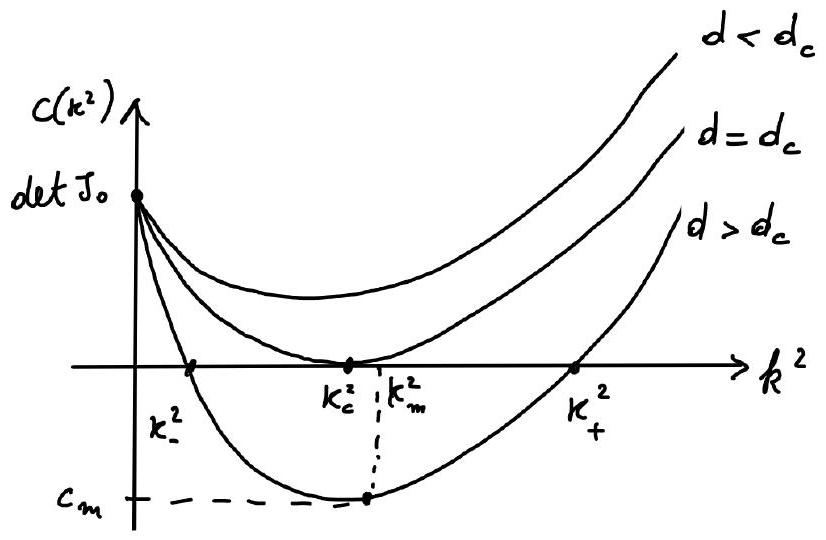
\includegraphics[width=0.5\textwidth]{2025_10_17_3cf351a4349ae3691080g-09}
\end{center}
critical diffusivities ratio for Turing pottems to emerge.

Gitical ratio ( $d_{c}$ )
At the bifurcation $C_{\text {min }}=0$, which can be obtained only when $D_{1}$ and $D_{2}$ have a specific satio. From ep. (20) and $\frac{D_{2}}{D_{1}}=d$ we get

$$ 
\left(d \partial_{u} f+\partial_{v} g
ight)^{2} \geqslant 4 d \operatorname{det} J_{0}>0
$$ 

So the enitical ratio $d_{c}$ of diffurivites satisfies the equation

$$ 
d_{c}^{2}\left(\partial_{u} f
\right)^{2}+\left(\partial_{v} g
\right)^{2}+2 d \partial_{u} f \partial_{v} g-4 d\left(\partial_{u} f \partial_{v} g-\partial_{v} f \partial_{u} g
\right)=0
$$ 

02
(21)

$$ 
d_{c}^{2}\left(\partial_{u} f
\right)^{2}+2
\left(2 \partial_{v} f \partial_{u} g-\partial_{u} f \partial_{v} g
\right) d_{c}+\left(\partial_{v} g
\right)^{2}=0
$$ 

From $d_{c}$ we can calculate the critical wavenumber $k_{c}^{2}$. Indeed from ep. (19)

$$ 
k_{\text {min }}^{2}=\frac{D_{2} \partial_{u} f+D_{1} \partial_{v} g}{2 D_{1} D_{2}}=\frac{1}{D_{1}} \frac{d \partial_{u} f+2 g}{2 d}=\frac{1}{D_{1}} \sqrt{\frac{\operatorname{det}
\left(J_{0}
ight)}{d}}
$$ 

from ey, (18) with $c_{\text {min }}=0$
from which we obtain (when $c_{\text {min }}=0, k_{\text {min }}=k_{c}$ ):
(22) $k_{c}^{2}=\frac{1}{D_{1}} \sqrt{\frac{\operatorname{det}
\left(J_{0}
ight)}{d_{c}}}$ where $d_{c}$ is from (21).

Conditions for Turing potterns to emerge:
Conditions (14), (15) and (20) ensure that the spatially uniform state is linearly stoble but has at least one wave number $k$ for which $\lambda
\left(k^{2}
\right)$ has paritive real part.
When we impose fero-flut boundary conditions, wavenumbers are restricted to $k=\frac{n \pi}{L}$. Therefore there must exist at least one integer volue $n=1,2 \ldots$ for which $c
\left(k^{2}
\right)<0$ (in this cose $d>d_{c}$ ). In this case the range of unstable wavemumbers is obtained from the feros $k_{ \pm}^{2}$ of $c
\left(k^{2}
\right)=0$ (see ey. (17). We get
(22) $\quad k_{ \pm}^{2}=\frac{D_{2} \partial_{u} f+D_{1} \partial_{v} g \pm \sqrt{\left(D_{2} \partial_{u} f+D_{1} \partial_{v} g
\right)^{2}-4 D_{1} D_{2}\left(\partial_{u} f \partial_{v} g-\partial_{v} f \partial_{u} g
\right)}}{2 D_{1} D_{2}}$
(23) $\quad k_{-}^{2} \leqslant\left(\frac{n \pi}{L}
\right)^{2} \leqslant k_{+}^{2}$
see also the previous figure and this one
\begin{center}
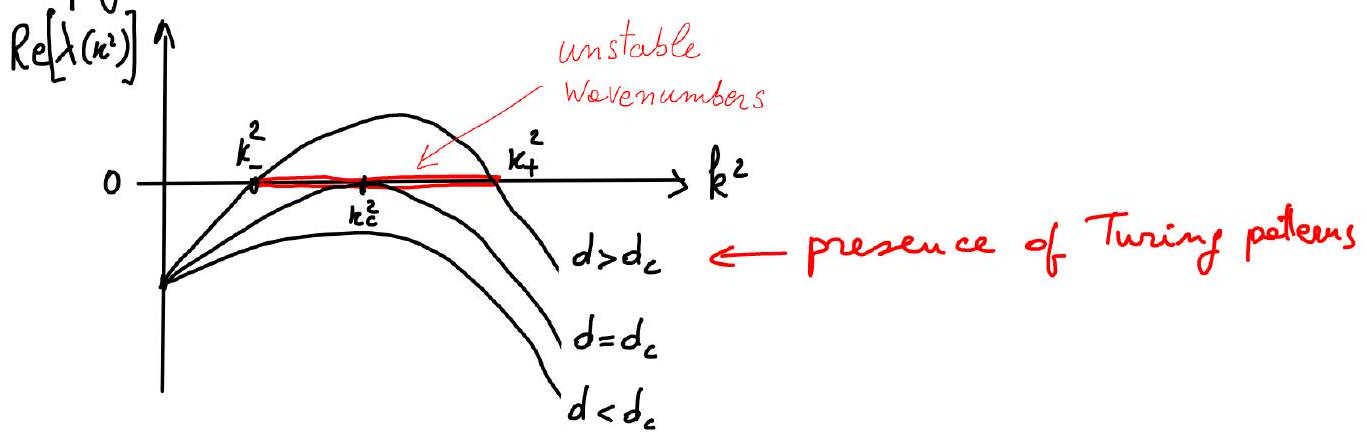
\includegraphics[width=0.5\textwidth]{2025_10_17_3cf351a4349ae3691080g-10}
\end{center}

Important comments :

\begin{enumerate}
  item Because $\partial_{u} f+\partial_{v g}<0$ ( $\varphi$. (14)) and $D_{2} \partial_{u} f+D_{1} \partial_{v} g>0$ (eq. (20), it follows that $\partial_{n} f$ and $\partial_{r} g$ must be of opposite sign.
If we take $\partial_{u} f>0$ (activator) and $\partial_{v} g<0$ (inhibitor) we get $\partial_{u} f<\left|\partial_{v} g
\right|$. From el. (20) we have $D_{2} \partial_{n} f+D_{1} \partial_{v} g>0$, thes (t)
\end{enumerate}


\begin{equation*} 
\frac{D_{2}}{D_{1}}>-\frac{\partial_{v} g}{\partial_{n} f}=\frac{\left|\partial_{v} g
\right|}{\partial_{n} f}>1 \Rightarrow D_{2}>D_{1} \tag{24}
\end{equation*} 

from ( $A$ )
This is usually summerifed by saying that
The inhibitor must diffuse faster than the activator.
(2) From ep. (14) $\left(T_{2}
\left(J_{0}
\right)<0
\right)$, (15) ( $\operatorname{det} J_{0}>0$ ) and ep. (20), it follows that $J_{0}$ must take one of the two forms: ( $u$ activ., $v$ inhib.)
\begin{center}
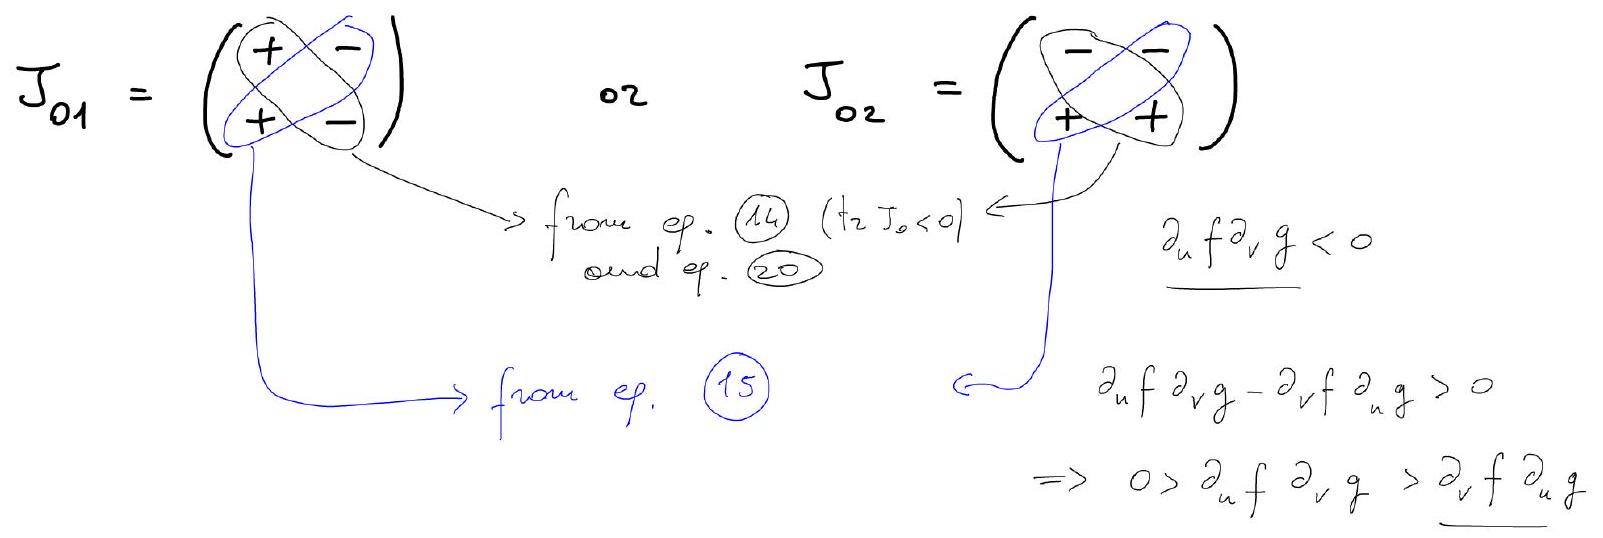
\includegraphics[width=0.5\textwidth]{2025_10_17_3cf351a4349ae3691080g-11}
\end{center}
on the alternative ones (vactiv., $u$ imhib.)

$$ 
J_{03}=-J_{01}=\binom{-+}{-+} \quad J_{04}=-J_{02}=\binom{++}{--}
$$ 

for allowing the emergence of a Tursing pottern.
(3) When the linearized equations (ree ep. (8)) at $\left(u_{0}, v_{0}
\right)$ have $J_{0}$ of the form $J_{01}$, we say that the system is a pure activator--imhibitor system. From ep. (8) and Jor
\begin{center}
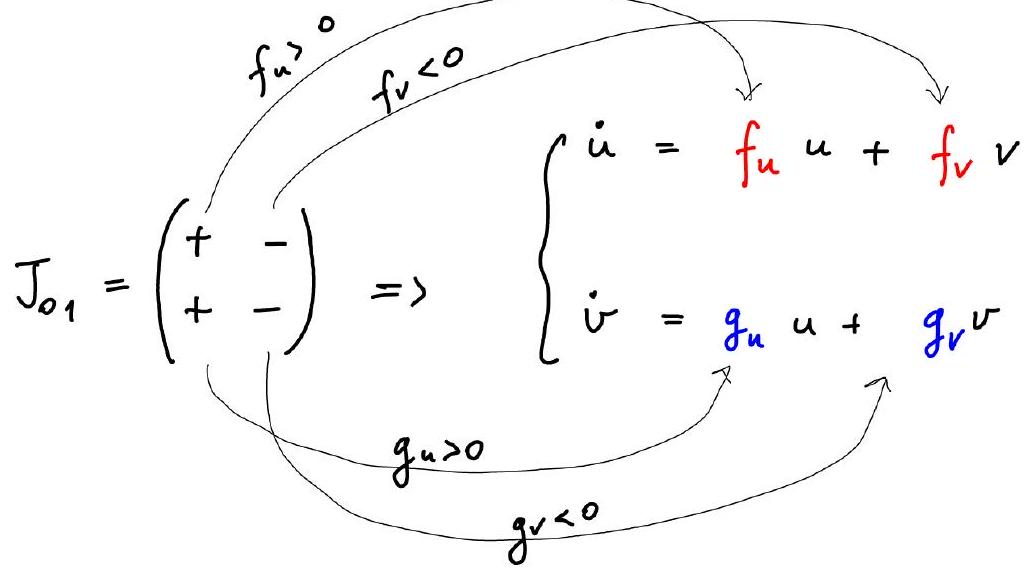
\includegraphics[width=0.5\textwidth]{2025_10_17_3cf351a4349ae3691080g-12(4)}
\end{center}
\begin{center}
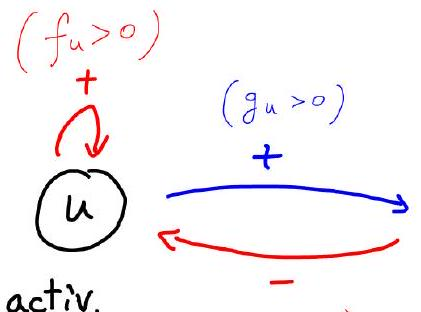
\includegraphics[width=0.5\textwidth]{2025_10_17_3cf351a4349ae3691080g-12}
\end{center}
(a) At steady state $u$ activates its own production, but $v$ inhibits the production of $u$;
(b) At steady state $u$ also activates the production of $v$, but $v$ intuibits its own production.

The equations and diagnam show why $u$ is termed ACTIVATOR, while $v$ is termed INHIBITOR. Beconse we also have $D_{2}>D_{1}$ we get short-range activation and long-rage inhibition.

In this cose $u$ and $v$ grow in phase: (look at the eigenvectors of $J_{01}$ )
\begin{center}
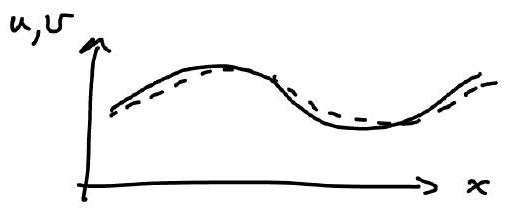
\includegraphics[width=0.5\textwidth]{2025_10_17_3cf351a4349ae3691080g-12(1)}
\end{center}

In the second cose for $J_{02}$ :
\begin{center}
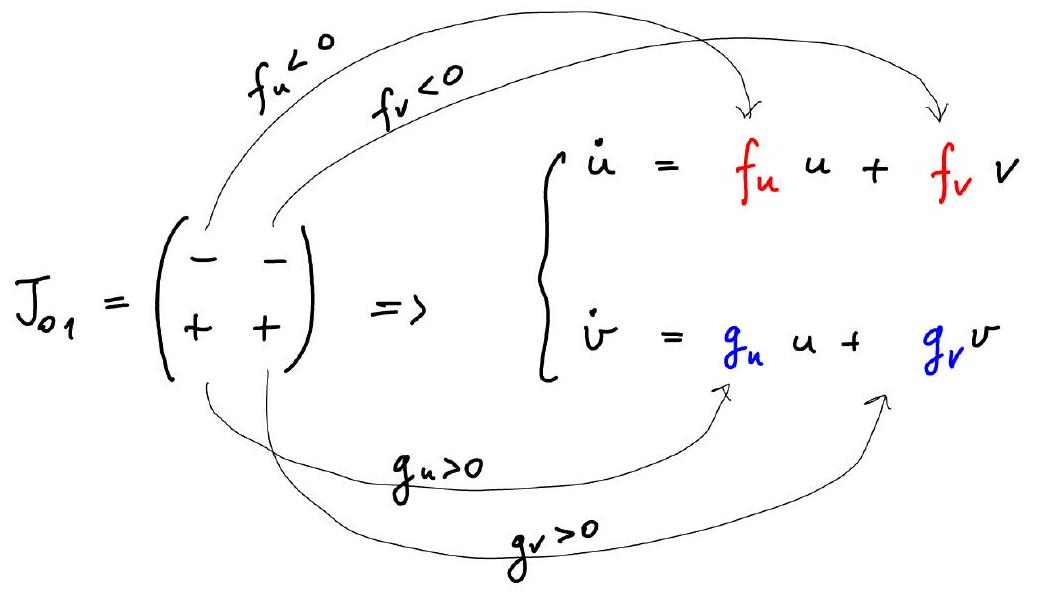
\includegraphics[width=0.5\textwidth]{2025_10_17_3cf351a4349ae3691080g-12(3)}
\end{center}
\begin{center}
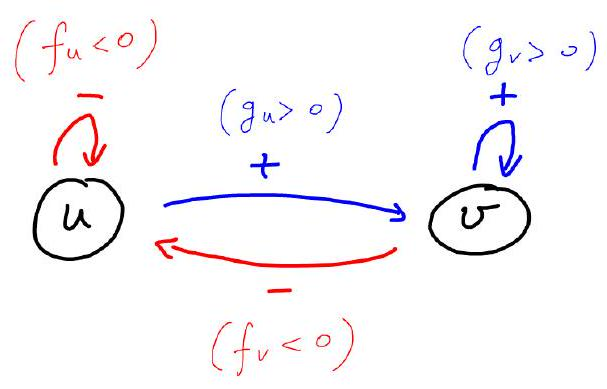
\includegraphics[width=0.5\textwidth]{2025_10_17_3cf351a4349ae3691080g-12(2)}
\end{center}
(c) At steody state, $u$ inhibits its own production as well as $v$ imhibits the production of $u$;
(c) At stady state, $u$ produces $v$, and $v$ activates itself.

In this case the system is called cress-activator-inhibitor system and $u$ and $v$ grow out of phase ( $180^{\circ}$ )
\begin{center}
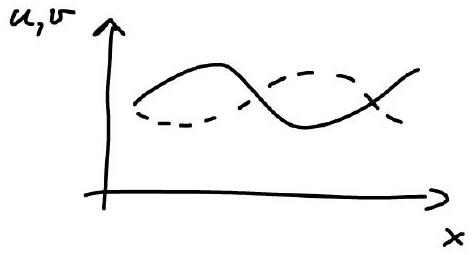
\includegraphics[width=0.5\textwidth]{2025_10_17_3cf351a4349ae3691080g-13}
\end{center}
(4) From ep. (23) it follows that there exists a minimum doursin size for pottern formation. Indeed, for $L$ sufficiently small, the inequality in (23) connot be satisfied for $n>0$.
(5) As the domain size increases ( $L$ becomes lager), the number of vioble integers also increases and the pattern will become more complicated.
(6) Considerotions in (3) and (4) con be extended to higher chimensions, where there may occur degeneracy. In $d=2$

$$ 
k^{2}=\left(\frac{m \pi}{L_{x}}\right)^{2}+\left(\frac{m \pi}{L_{y}}\right)^{2} \quad n, m \in \mathbb{N}
$$ 

Because there may exist multiple pains ( $n, m$ ) which produce the same $k^{2}$, in higher dimensions different patterns (say, stripes, chenboard, spots..) may emerge due to different initial conditions, which may combine different solutions (on the boxis of the non-limear terms).